

\newthought{The main purpose }~of this study is to investigate the dynamics of mesoscale ocean eddies on a global scale, \ie to provide a statistical census on horizontal scale, lifetime and zonal drift speeds.
%\newthought{The main purpose }~of this study is to investigate the dynamics, in particular horizontal scales and zonal translational speeds, of geostrophic mesoscale ocean eddies on a global scale.
By virtue of the geostrophic character of the scales of concern, such vortices implicate a local upheaval/depression of density surfaces, usually also including the sea surface \footnote{As in theory, baroclinic eddies have most of their energy in the first (surface-intensified) baroclinic mode \citep{olbers2012ocean}.}.
\begin{wrapfigure}{r}{.6\textwidth}
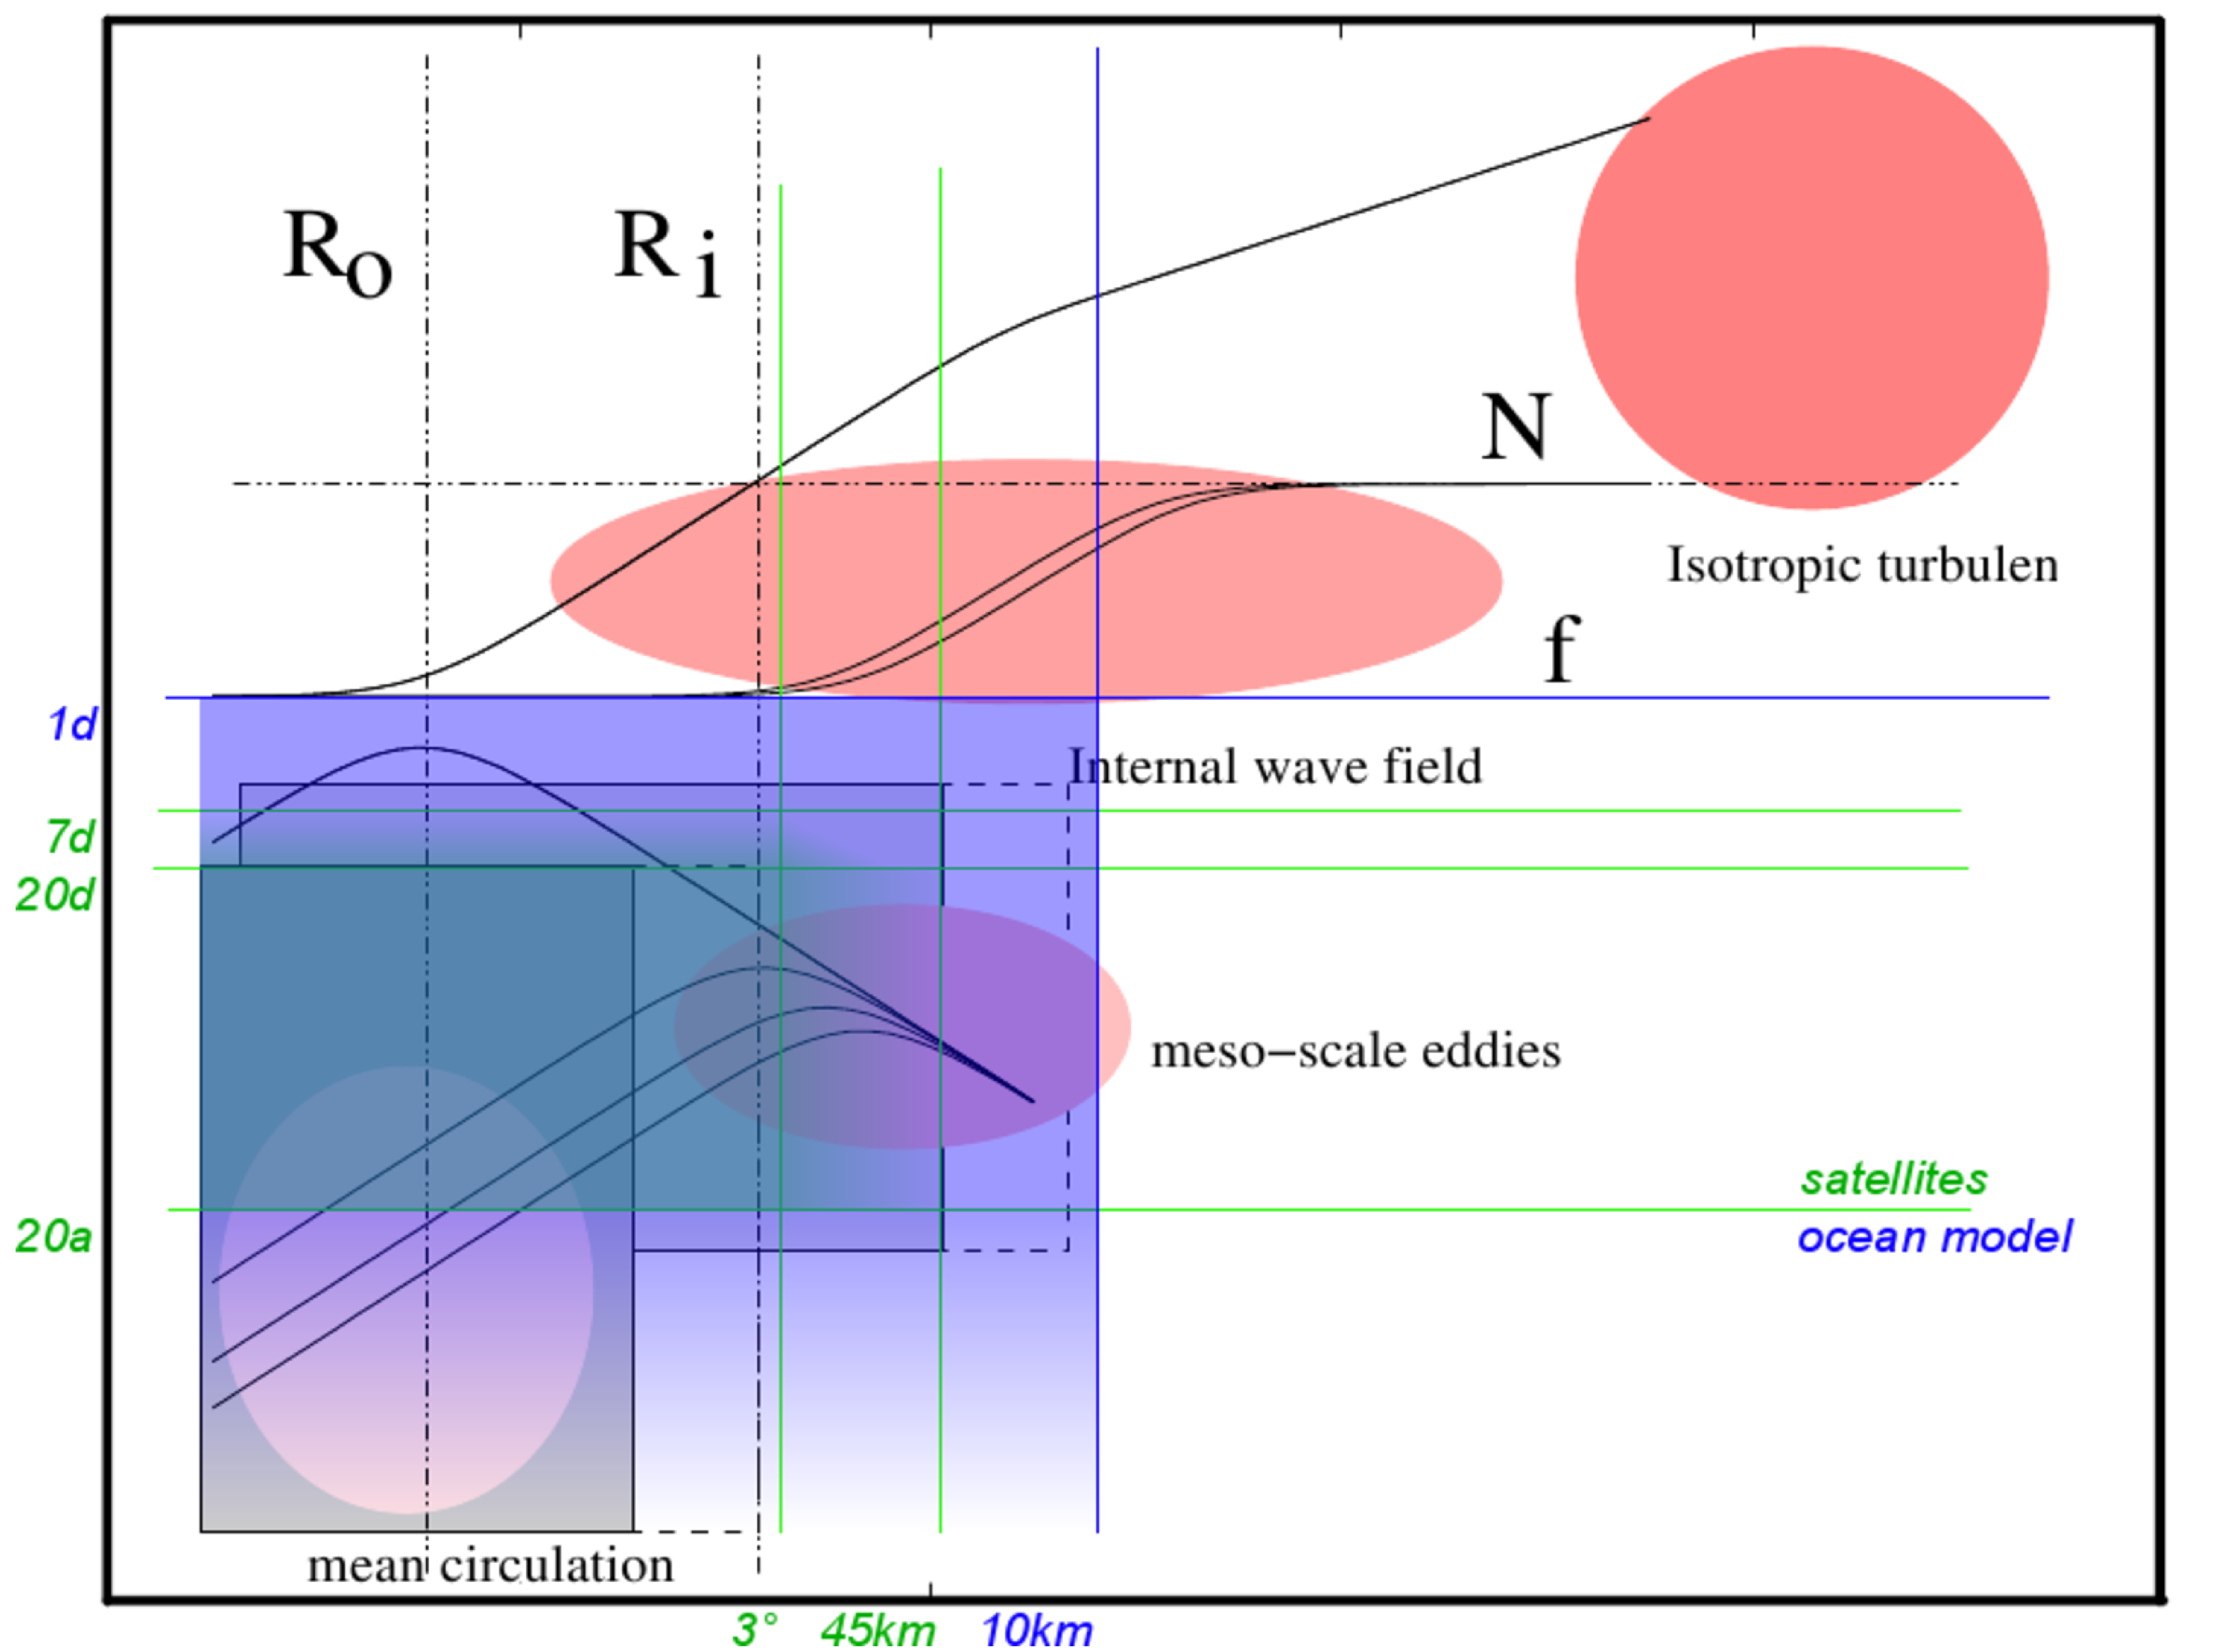
\includegraphics[width=0.6\textwidth]{scales}
\caption{Resolutions for model vs satellite. Modified version from \citet{olbers2012ocean}.}
\label{fig:scales}
\end{wrapfigure}
 The resultant \textit{hills} and \textit{valleys} in surface anomaly can be resolved by combining multiple satellite-altimetry signals (see \cref{fig:scales}). One motivation of this study is to investigate whether the resolutions in space and time of such altimeter-derived products suffice to successfully track individual eddies over long periods of time and to precisely determine their horizontal extent and drift speed. The detection/tracking/analyzing procedure of individual eddies is done globally via an automated parallelized computer-program. 
To analyze the effects of different time/space-resolutions, a finer-grid \SSH-product of a modern ocean-circulation model is subjected to the algorithm as well.
Due to the inherently technical character of the matter, large parts of this text are dedicated to details of the algorithm \footnote{see the \cref{chap:algorithm}.}. Oceanographic results are treated in the \href{chap:results}{results}- and \href{chap:discussion}{discussion}-chapters. This chapter discusses the physics of mesoscale geostrophic turbulence and introduces a handful of relevant historical papers. Since focus is on horizontal scales, drift speeds and the comparison of results between the \AVI~product and \SSH-data from the \POP~ocean model, sections generally focus on either of these three topics.

%\newthought{The main purpose }  of this study is to create a computer program that is able to \textbf{detect}, \textbf{track} and \textbf{analyze} mesoscale ocean eddies via their surface signal in sea-surface-height (SSH).
